\documentclass[
	12pt,
	a4paper,
	bibtotoc,
	cleardoubleempty, 
	idxtotoc,
	openright
	final,
	listof=nochaptergap,
	]{scrbook}

\usepackage[T1]{fontenc}
\usepackage{times}
\usepackage[utf8]{inputenc}
\fontfamily{ptm}\selectfont

% ##################################################
% Unterstuetzung fuer die deutsche Sprache
% ##################################################
\usepackage[ngerman]{babel}
\usepackage[ngerman=ngerman-x-latest]{hyphsubst}
\sloppy

% ##################################################
% Dokumentvariablen
% ##################################################

% Persoenliche Daten
\newcommand{\docNachnamed}{Schlageter}
\newcommand{\docVornamed}{Daniel}
\newcommand{\docNachnamec}{Petrusic}
\newcommand{\docVornamec}{Daniel}
\newcommand{\docNachname}{Hertfelder}
\newcommand{\docVorname}{Kevin}
\newcommand{\docNachnameb}{Kroner}
\newcommand{\docVornameb}{Patrick}
\newcommand{\docNachnamea}{Kienzler}
\newcommand{\docVornamea}{Stefan}


% Dokumentdaten
\newcommand{\docTitle}{SensorCar OpenPEARL}
%\newcommand{\docUntertitle}{} % Kein Untertitel
\newcommand{\docUntertitle}{Semesterprojekt WS17/18}
% Arten der Arbeit: Bachelorthesis, Masterthesis, Seminararbeit, Diplomarbeit
\newcommand{\docArtDerArbeit}{Dokumentation}
%Studiengaenge: Allgemeine Informatik Bachelor, Computer Networking Bachelor,
% Software-Produktmanagement Bachelor, Advanced Computer Scinece Master
\newcommand{\docStudiengang}{AIN}
\newcommand{\docAbgabedatum}{18.12.2017}
\newcommand{\docErsterReferent}{Prof. Dr. Rainer Müller}
%\newcommand{\docZweiterReferent}{-} % Wenn es nur einen Betreuer gibt
\newcommand{\docZweiterReferent}{-}

% ##################################################
% Allgemeine Pakete
% ##################################################

% Abbildungen einbinden
\usepackage{graphicx}

% Zusaetsliche Sonderzeichen
\usepackage{dingbat}

% Farben
\usepackage{color}
\usepackage[usenames,dvipsnames,svgnames,table]{xcolor}

% Maskierung von URLs und Dateipfaden
\usepackage[hyphens]{url}

% Deutsche Anfuehrungszeichen
\usepackage[babel, german=quotes]{csquotes}

% Pakte zur Index-Erstellung (Schlagwortverzeichnis)
\usepackage{index}
\makeindex

% Ipsum Lorem
% Paket wird nur für das Beispiel gebraucht und kann gelöscht werden
\usepackage{lipsum}

% ##################################################
% Seitenformatierung
% ##################################################
\usepackage[
	portrait,
	bindingoffset=1.5cm,
	inner=2.5cm,
	outer=2.5cm,
	top=3cm,
	bottom=2cm,
	%includeheadfoot
	]{geometry}

% ##################################################
% Kopf- und Fusszeile
% ##################################################

\usepackage{fancyhdr}

\pagestyle{fancy}
\fancyhf{}
\fancyhead[EL,OR]{\sffamily\thepage}
\fancyhead[ER,OL]{\sffamily\leftmark}

\fancypagestyle{headings}{}

\fancypagestyle{plain}{}

\fancypagestyle{empty}{
  \fancyhf{}
  \renewcommand{\headrulewidth}{0pt}
}

%Kein "Kapitel # NAME" in der Kopfzeile
\renewcommand{\chaptermark}[1]{
	\markboth{#1}{}
   	\markboth{\thechapter.\ #1}{}
}

% ##################################################
% Schriften
% ##################################################

% Stdandardschrift festlegen
\renewcommand{\familydefault}{\sfdefault}

% Standard Zeilenabstand: 1,5 zeilig
\usepackage{setspace}
\onehalfspacing 

% Schriftgroessen festlegen
\addtokomafont{chapter}{\sffamily\large\bfseries} 
\addtokomafont{section}{\sffamily\normalsize\bfseries} 
\addtokomafont{subsection}{\sffamily\normalsize\mdseries} 
\addtokomafont{caption}{\sffamily\normalsize\mdseries} 

% ##################################################
% Inhaltsverzeichnis / Allgemeine Verzeichniseinstellungen
% ##################################################

\usepackage{tocloft}

% Punkte auch bei Kapiteln
\renewcommand{\cftchapdotsep}{3}
\renewcommand{\cftdotsep}{3}

% Schriftart und -groesse im Inhaltsverzeichnis anpassen
\renewcommand{\cftchapfont}{\sffamily\normalsize}
\renewcommand{\cftsecfont}{\sffamily\normalsize}
\renewcommand{\cftsubsecfont}{\sffamily\normalsize}
\renewcommand{\cftchappagefont}{\sffamily\normalsize}
\renewcommand{\cftsecpagefont}{\sffamily\normalsize}
\renewcommand{\cftsubsecpagefont}{\sffamily\normalsize}

%Zeilenabstand in den Verzeichnissen einstellen
\setlength{\cftparskip}{.5\baselineskip}
\setlength{\cftbeforechapskip}{.1\baselineskip}

% ##################################################
% Abbildungsverzeichnis und Abbildungen
% ##################################################

\usepackage{caption}

\usepackage{wrapfig}

% Nummerierung von Abbildungen
\renewcommand{\thefigure}{\arabic{figure}}
\usepackage{chngcntr}
\counterwithout{figure}{chapter}

% Abbildungsverzeichnis anpassen
\renewcommand{\cftfigpresnum}{Abbildung }
\renewcommand{\cftfigaftersnum}{:}

% Breite des Nummerierungsbereiches [Abbildung 1:]
\newlength{\figureLength}
\settowidth{\figureLength}{\bfseries\cftfigpresnum\cftfigaftersnum}
\setlength{\cftfignumwidth}{\figureLength}
\setlength{\cftfigindent}{0cm}

% Schriftart anpassen
\renewcommand\cftfigfont{\sffamily}
\renewcommand\cftfigpagefont{\sffamily}

% ##################################################
% Tabellenverzeichnis und Tabellen
% ##################################################

% Nummerierung von Tabellen
\renewcommand{\thetable}{\arabic{table}}
\counterwithout{table}{chapter}

% Tabellenverzeichnis anpassen
\renewcommand{\cfttabpresnum}{Tabelle }
\renewcommand{\cfttabaftersnum}{:}

% Breite des Nummerierungsbereiches [Abbildung 1:]
\newlength{\tableLength}
\settowidth{\tableLength}{\bfseries\cfttabpresnum\cfttabaftersnum}
\setlength{\cfttabnumwidth}{\tableLength}
\setlength{\cfttabindent}{0cm}

%Schriftart anpassen
\renewcommand\cfttabfont{\sffamily}
\renewcommand\cfttabpagefont{\sffamily}

% Unterdrueckung von vertikalen Linien
\usepackage{booktabs}

% ##################################################
% Listings (Quellcode)
% ##################################################

\usepackage{listings}
\lstset{
	language=java,
	backgroundcolor=\color{white},
	breaklines=true,
	prebreak={\carriagereturn},
 	breakautoindent=true,
 	numbers=left,
 	numberstyle=\tiny,
 	stepnumber=2,
 	numbersep=5pt,
 	keywordstyle=\color{blue},
   	commentstyle=\color{green},   
   	stringstyle=\color{gray}
}
  	
% ##################################################
% Theoreme
% ##################################################
  	
% Umgebung fuer Beispiele
\newtheorem{beispiel}{Beispiel}

% Umgebung fuer These
\newtheorem{these}{These}

% Umgebung fuer Definitionen
\newtheorem{definition}{Definition}
  	
% ##################################################
% Literaturverzeichnis
% ##################################################

\usepackage{natbib}

% ##################################################
% Abkuerzungsverzeichnis
% ##################################################

\usepackage[printonlyused]{acronym}

% ##################################################
% PDF / Dokumenteninternelinks
% ##################################################

\usepackage[
	colorlinks=false,
   	linkcolor=black,
   	citecolor=black,
  	filecolor=black,
	urlcolor=black,
    bookmarks=true,
    bookmarksopen=true,
    bookmarksopenlevel=3,
    bookmarksnumbered,
    plainpages=false,
    pdfpagelabels=true,
    hyperfootnotes,
    pdftitle ={\docTitle},
    pdfauthor={\docVornamed~\docNachnamed},
    pdfcreator={\docVornamed~\docNachnamed}]{hyperref}

\begin{document}

\setcounter{secnumdepth}{3}

% Titelblatt
\begin{titlepage}
\pagestyle{empty}

% ##################################################
% HFU-Logo einbinden
% ##################################################
\begin{flushright}
\begin{figure}[ht]
\flushright

\includegraphics[height=3cm]{content/pictures/hfu.jpg}
\end{figure}
\end{flushright}

% ##################################################
% Titel
% ##################################################
\begin{center}
{\fontsize{18}{22} \selectfont \docArtDerArbeit}\\[5mm]
\vspace{1cm}
\begin{onehalfspace}
{\fontsize{22}{26} \selectfont \textbf{\docTitle}}\\[5mm]
{\fontsize{18}{22} \selectfont \docUntertitle}


\end{onehalfspace}
\end{center}

% ##################################################
% Zusatzinformationen
% ##################################################
\vfill
\begin{center}
\begin{tabular}{lcl}
Referent  		&:& \textsc{\docErsterReferent} 	\\ \\
Korreferent 		&:& \docZweiterReferent \\ \\	
Vorgelegt am 	&:& \docAbgabedatum 	\\ \\
Vorgelegt von 	&:& \textsc{\docVorname~\docNachname}\\
				& & \textsc{\docVornamea~\docNachnamea}\\
				& & \textsc{\docVornameb~\docNachnameb}\\
				& & \textsc{\docVornamec~\docNachnamec}\\
				& & \textsc{\docVornamed~\docNachnamed}\\			
\end{tabular}
\end{center}
\end{titlepage}
\cleardoubleemptypage

\frontmatter



% Inhaltsverzeichnis

\tableofcontents
\addcontentsline{toc}{chapter}{Inhaltsverzeichnis}

\cleardoubleemptypage


% Inhalt
\mainmatter

\chapter{Einleitung}

	Das Semesterprojekt OpenPEARL im Wintersemester 2017/18 beschäftigt sich mit der Anwendung von OpenPEARL insbesondere im Zusammenhang mit Sensorik. 
	
	\section{OpenPEARL}
	PEARL steht für \emph{Process and Experiment Automation Realtime Language}, eine höhere Programmiersprache, die speziell dafür entworfen wurde, Multitaskingaufgaben bei der Steuerung technischer Prozesse zu steuern. Die Sprache wurde um 1975 am IRT Institut der Leibniz Universität in Hannover entwickelt und 1998 vom Deutschen Institut für Normung in der DIN66253-2 standardisiert (http://pearl90.de).\\
	OpenPEARL ist eine quelloffene Implementierung eines Compilers und einer Laufzeitumgebung für PEARL. OpenPEARL befindet sich aktuell noch in der Entwicklung, ist aber weit genug fortgeschritten, um erste Beispielprojekte damit umzusetzen. In dieser Dokumentation werden deshalb auch in OpenPEARL gefundene Fehler festgehalten.
	
	\section{Projektziel}
	Ziel des Projektes ist es, das OpenPEARL-System bei der Ansteuerung verschiedenartiger Peripheriegeräte zu testen. Die verschiedenen Sensoren und Aktoren sollen auf ihre Nutzbarkeit mit OpenPEARL allgemein und in einem größeren OpenPEARL-Projekt im Speziellen überprüft werden. Als Plattform wird ein Raspberry Pi 3 genutzt. \\
	Als Gesamtsystem soll ein autonomes Modellauto entstehen, das, mit ebenjenen Sensoren ausgestattet, nach Möglichkeit einer Linie folgen und auf Abruf weitere Manöver ausführen kann.
	
	\section{Über dieses Dokument}
	Diese Dokumentation beschreibt die Planung, Struktur und die Ergebnisse des Projektes. Sie beschreibt nicht das vollständige Vorgehen oder alle genutzten Informationen, sondern beschreibt die Ergebnisse unter Erwähnung wichtiger Ereignisse und mit Verweisen auf genutzte Quellen. \\
	Der Programmcode sowohl für einzelne Module als auch für das Gesamtsystem ist in einem öffentlichen \href{https://github.com/OpenPearl-HFUWPV1718/SensorCar}{Git-Repository} abgelegt, auf das hier und an geeigneter Stelle verwiesen wird. Der Programmcode ist dokumentiert und nicht Teil dieses Dokumentes, stattdessen werden in diesem Dokument die zugrundeliegenden Ideen erläutert, die notwendig sind, um den dokumentierten Code vollständig zu verstehen.
	
	
	
\chapter{Funktionsbeschreibung}
\label{funktionsbeschreibung}

In diesem Kapitel wird die Funktionalität des Gesamtsystems, an der sich die Auswahl und dann gewissermaßen auch das Vorgehen bei der Inbetriebnahme der einzelnen Komponenten orientiert, kurz beschrieben.

\section{Grundfunktionalität}
Das OpenPEARL SensorCar ist ein mit zwei Motoren und unterschiedlichen Sensoren ausgestattetes Modellauto. Die Sensoren sollen verschiedene Signale aufnehmen, verarbeiten und anzeigen, die Schrittmotoren sollen das Fahren in verschiedenen Geschwindigkeiten und Richtungen ermöglichen.
Es werden folgende Komponenten eingesetzt:\\

\begin{itemize}
	\item \textbf{Raspberry Pi mit OpenPEARL}: Kernkomponente des SensorCar ist ein Raspberry Pi, auf dem ein OpenPEARL Programm läuft, das alle angeschlossenen Sensoren und Aktoren verwaltet und steuert.
	\item \textbf{Schrittmotor}: Zwei Schrittmotoren steuern jeweils zwei über ein Gummi verbundene Räder (ein Motor für eine Seite). Dadurch lässt sich das Auto mit unterschiedlichen Geschwindigkeiten sowohl vorwärts wie auch rückwärts bewegen und Kurven mit beliebigen Radius fahren.
	\item \textbf{Lichtrechen}: Ein Lichtrechen, bestehend aus mehreren binären Helligkeitssensoren, erfasst den Untergrund in zwei Helligkeitsstufen. 
	\item \textbf{Modellauto}: Alle Komponenten werden auf einem selbstgedruckten Modellauto aufgebracht.
	\item \textbf{Farbsensor}: Ein Farbsensor kann farbige Punkte auf dem Boden erfassen und verschiedene Aktionen einleiten.
	\item \textbf{Beleuchtung}:
		\subitem Weiße LEDs: Zwei weiße LEDs dienen als Frontscheinwerfer.
		\subitem Rote LEDs: Zwei rote LEDs dienen als Rückleuchten.
		\subitem Gelbe LEDs: Vier gelbe LEDs dienen als Blinker.
\end{itemize}

\section{Erweiterte Funktionalität}
Zusätzlich zum eingabegesteuerten Fahren soll das SensorCar nach Möglichkeit selbstständig einer schwarzen Linie folgen und verschiedene Aktionen (Anhalten, Geradeausfahren) auf Abruf -- durch Erkennung von Farbpunkten auf der Linie -- durchführen können.

\section{Kommunikation}
Aktuelle Informationen über das SensorCar können über einen Browser mittel einer \emph{http} Anfrage abgefragt werden. Dazu läuft in OpenPEARL ein Webserver, der die Informationen abfragt und ausgibt.\\
Eingehende Kommunikation erfolgt über ssh.





\chapter{Projektverlauf}
	
	\section{Organisation}
	
	Das Projektteam besteht aus den fünf Mitgliedern Kevin Hertfelder, Stefan Kienzler, Patrick Kroner, Daniel Petrusic und Daniel Schlageter. Betreut wird das Projekt durch Herrn Prof. Dr. Rainer Müller. In wöchentlichen Projekttreffen wird er aktuelle Status festgehalten und die Aufgaben für die nächste Woche, gemäß angepasster Planung, festgelegt. Die Protokolle dieser Sitzungen können im \href{https://github.com/OpenPearl-HFUWPV1718/SensorCar}{Repository} eingesehen werden.\\
	
	
	\section{Struktur}
	Das Projekt gliedert sich, entsprechend des oben beschriebenen Ziels, in mehrere Teilprojekte:
	
	\begin{itemize}
		\item \textbf{Projektstart}\\
		Einführung in das Projekt und Festlegung der Organisation. Grundlegende Abstimmung über Ziel und Umfang.
		\item \textbf{Einführung OpenPEARL und Philosophenproblem}\\
		 Zur Einarbeitung in die Programmiersprache OpenPEARL implementiert das Projektteam jeweils das Philosophenproblem.
		\item \textbf{Einrichtung der Raspberry Pis}\\
		 Für die weitere Arbeit am Projekt werden zwei Rasperberry Pi 3 eingerichtet, um mit OpenPEARL und NFS zu arbeiten. Der Zugriff auf die Rechner soll mittels \emph{ssh} möglich sein.
		\item \textbf{Inbetriebnahme und Test der Hardwarekomponente}\\  Die einzelnen Komponenten (Sensoren und Aktoren) werden als Teilprojekte separat am Raspberry Pi in Betrieb genommen und getestet.
		\item \textbf{Entwurf und Druck des Modells}\\
		Das Modell für den mechanischen Aufbau wird entwickelt und mit dem 3D-Drucker ausgedruckt und getestet.
		\item \textbf{Detailplanung des Gesamtsystems}\\  Die genaue Funktionalität und der Hardwareaufbau des Gesamtsystems werden festgelegt und dokumentiert.
		\item \textbf{Zusammensetzung Gesamtsystems}\\
		Nachdem alle Komponenten erfolgreich in Betrieb genommmen und getestet wurden, wird das Gesamtsystem im Sinne des Ziels zusammengebaut. Daraufhin wird die Funktionalität des Gesamtsystems programmiert. Im Sinne eines inkrementell iterativen Vorgehens erfolgen Anforderungsanalyse, Implementierung und Tests bis das System die Anforderungen erfüllt.
		\item \textbf{Projektabschluss}\\
		Zum Abschluss des Projekts erfolgt die Fertigstellung der Dokumentation und Abnahme des Ergebnisses.
		\item \textbf{Projektvorstellung}\\
		Das Ergebnis des Projektes wird im Rahmen der Projektpräsentationen vorgestellt.
	\end{itemize}

	\section{Ablauf}
	Tabelle \ref{tab:zeitplan} detailliert die grobe Zeitplanung für den Projektablauf. Änderungen sind vorbehalten.\\
	
	\begin{table}[H]
		
		\begin{center}
			\renewcommand{\arraystretch}{1.2}
			\begin{tabular}{|p{5cm}|l|}
				\hline
				\textbf{Zeitraum} & \textbf{Teilprojekt / Aufgabe}\\
				\hline
				09.10.17 -- 16.10.17 & Projektstart\\
				\hline
				16.10.17 -- 23.10.17 & Einführung in OpenPEARL und Philosophenproblem\\
				\hline
				23.10.17 -- 30.10.17 & Einrichtung der Raspberry Pis\\
				\hline
				30.10.17 -- 11.12.17 & Inbetriebnahme und Test der Hardwarekomponenten\\
				\hline
				30.10.17 -- 18.12.17 & Entwurf und Druck des Modells\\
				\hline
				11.12.17 -- 15.01.18 & Zusammensetzung des Gesamtsystems\\
				\hline 
				15.01.18 -- 22.01.18 & Projektabschluss\\
				\hline
				26.01.18 & Projektpräsentation\\
				\hline
			\end{tabular}
		\end{center}
		\caption{Zeitplan}\label{tab:zeitplan}
	\end{table}
	
\chapter{Philosophenproblem}

Um mit der Sprache OpenPEARL und ihren Konstrukten insbesondere zur Nebenläufigkeit vertraut zu werden, wurde als einführendes Beispiel das Philosophenproblem gelöst.

\section{Das Philosophenproblem}
	Das Philosophenproblem ist ein bekanntes Fallbeispiel für Nebenläufigkeit und Verklemmung. Fünf Philosophen sitzen um einen runden Tisch, jeder der Philosophen hat einen Teller mit Spaghetti vor sich. Um diese zu essen, benötigt jeder Philosoph zwei Gabeln, es sind jedoch nur fünf Gabeln, jeweils eine zwischen zwei Philosophen, vorhanden. Es können also nicht alle Philosophen gleichzeitig essen.\\
	Die Philosophen werden als Prozesse oder Threads betrachtet, die gleichzeitig auf mehrere Ressourcen, die Gabeln, zugreifen möchten.
	
\section{Umsetzung}
	Die Gabeln werden als Semaphoren realisiert. Diese bieten nur einer bestimmten Anzahl Threads bzw. im Kontext von OpenPEARL \emph{Tasks} die Möglichkeit der gleichzeitigen Belegung. Beim Philosophenproblem kann jede Gabel, also jede Semaphore, nur einmal belegt werden.\\
	Zum Essen benötigt ein Philosoph zwei Gabeln, also auch zwei Semaphoren. Erfolgt der Zugriff auf die Semaphoren nicht-atomar, das heißt voneinander getrennt und nacheinander, so kann es zur Verklemmung kommen: Jeder Philosoph hält eine Gabel und wartet auf die Freigabe der zweiten --- die Philosophen verhungern.\\
	OpenPEARL bietet zur einfachen Lösung des Problems die Möglichkeit, mehrere Semaphoren in einer atomaren Aktion gleichzeitig aufzunehmen. Dies ist nur dann erfolgreich, wenn alle Semaphoren belegbar sind, und verhindert eine Verklemmung.

\newpage

\section{Codebeispiel}
	Im Folgenden sind die relevanten Codeausschnitte einer Lösung des Philosophenproblems in OpenPEARL aufgeführt.
	
\subsection{Definition der Semaphoren}
	\begin{lstlisting}
! Semaphoren ("Gabeln"), die maximal ein mal (gleichzeitig) belegt werden koennen
DCL (g1, g2, g3, g4, g5) SEMA PRESET(1,1,1,1,1);
	\end{lstlisting}
	
\subsection{Aktivität eines Philosophen als Task}
	\begin{lstlisting}
philosopher1: TASK;
	REPEAT;
		! Gleichzeitige Anfrage fuer die Belegung der Semaphoren
		REQUEST g1, g2;
		PUT 'Philosopher 1 starts eating...' TO termout BY A, SKIP;
		AFTER timeone RESUME;
		PUT 'Philosopher 1 stops eating...' TO termout BY A, SKIP;
		! Gleichzeitige Freigabe der Semaphoren
		RELEASE g1, g2;
	END;
END;
	\end{lstlisting}
	
	Komplette Lösungen können im Ordner \emph{Code/Philosophenproblem} des \href{https://github.com/OpenPearl-HFUWPV1718/SensorCar}{Repositories} eingesehen werden.\\

\subsection{Kompilerfehler}
	Während der Implementierung des Philosophenproblems wurde ein Fehler im Kompiler entdeckt, der unter bestimmten Umständen das gleichezeitige Belegen zweier Semaphoren verhindert hat. Der Fehler wurde inzwischen behoben.
\chapter{Mechanischer Aufbau}
\section{Rahmenbedingungen}
Aufgrund des Vorhandenseins eines 3D-Druckers an der Hochschule und der damit verbundenen Flexibilität, haben wir uns entschlossen, das Gehäuse und die Halterungen für die einzelnen Komponenten zu drucken.
Allerdings gilt es auch hierbei einige Dinge zu beachten. Dadurch, dass der Drucker die Modelle schichtenweise von unten nach oben aufbaut, können beispielsweise Löcher in Wänden nur umständlich oder überhaupt nicht realisiert werden. Theoretisch kann dies durch ein Kippen des zu druckenden Körpers oder das Mitdrucken von Hilfselementen umgangen werden. In der Praxis und vor allem dann, wenn solche Probleme auf mehreren Seiten beziehungsweise an sehr filigranen Stellen eines Modells auftreten, nutzen auch diese Methoden nichts mehr.\\
Zudem kann das Innenleben der gedruckten Teile entweder durch eine Art Wabenstruktur oder komplett gefüllt aufgebaut sein. Durch den Aufbau in Form einer Wabenstruktur wird zum einen ein geringerer Verbrauch von Druckmaterialen und zum anderen eine wesentlich geringere Druckzeit erzielt. Vor allem der Zeitfaktor ist dabei nicht unrelevant, da selbst der Druck von einfachen und mittelgroßen Teilen in der Regel mehrere Stunden in Anspruch nimmt. Wenn man jedoch beabsichtigt die Komponenten zu verschrauben, oder ein sehr hohe Stabilität vorsieht, sollte man auf diese Druckart verzichten und einen gefüllten Druck vorziehen.\\
Um in dem Fall, dass ein Teil unseres Modells beschädigt wird, nicht alles erneut drucken zu müssen, ist das Gesamtmodell modular aufgebaut. Jedes Modul weißt entweder den weiblichen oder den männlichen Teil einer Steckverbindung auf.\\
Außerdem ist der Druckbereich eines 3D-Druckers beschränkt. Bei dem von uns genutzten 3D-Drucker sind wir vor allem auf einer der horizonzalen Achsen eingeschränkt. Der hier zur Verfügung stehende Druckbereich von maximal 21,4cm hat somit die Länge unseres Modells bestimmt.

\section{Motorenführung}
Da wir uns dazu entschlossen haben, jeweils beide Räder auf einer Seite über einen O-Ring miteinander zu verbinden, muss es eine möglichkeit geben, diese ein- und nachspannen zu können. Aus diesem Grund haben wir eine Art Schiene modelliert, in der ein Motor über jeweils eine Schraube mit zwei Muttern an der Vorder- sowie Hinterseite befestigt werden kann.
\begin{wrapfigure}[]{h}[4cm]{10cm}
	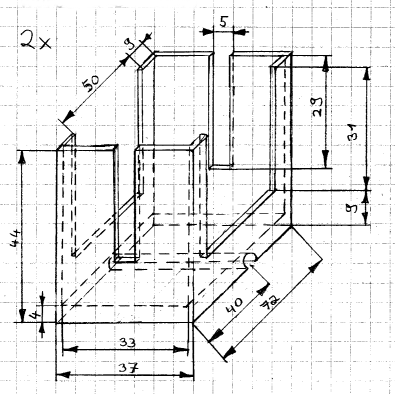
\includegraphics[width=6cm,angle=0]{content/pictures/motorenfuehrung.png}
\end{wrapfigure}
Sie weißt im Inneren eine effektive Länge von 68mm auf und erlaubt es uns somit je nach Größe der Muttern die Motoren mit einer Länge von 40mm um 15mm bis 20mm zu verstellen. Auf der hier gezeigten Skizze ist ein Schraubendurchmesser von 5mm vorgesehen. Dieser kann jedoch beliebig angepasst werden, wenn man die entsprechenden Maße der Motorenführung abändert. Über den weiblichen Teil einer Steckverbindung am unteren Ende wird die Motorenführung später seitlich mit später in der Dokumentation beschriebenen Bodenplatte verbunden.

\section{Motorenfassung}
Die Motoren werden jeweils in einer Halterung eingefasst, welche später in der Motorenführung beweglich gelagert sein wird, um die O-Ringe 
\begin{wrapfigure}[]{h}[4cm]{10cm}
	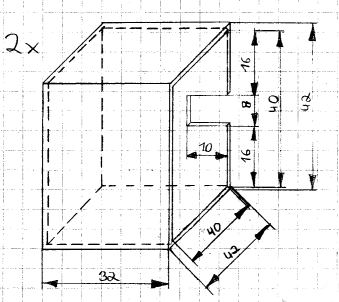
\includegraphics[width=6cm,angle=0]{content/pictures/motorenfassung.png}
\end{wrapfigure}
ein- und nachspannen zu können. Der Primärgrund für die Verwendung solcher Motorenfassungen ist jedoch der, dass die zu den Motoren gehörenden Treiberstufen über ein weiteres Bauteil an den Oberseiten der Motorenfassungen befestigt werden können. Auf diese Weise kann der für die Treiberstufen benötigte Platz auf der Bodenplatte eingespart werden. Zudem ist die Länge der Kabel zwischen Motor und Treiberstufe somit konstant. Um die Kabel, die seitlich aus den Motoren kommen zu berücksichtigen, befindet sich an einer Seite der Motorenfassungen eine entsprechende Aussparung.


\chapter{Komponenten}
\section{Raspberry Pi 3}
mit Anschlussplan...

\section{Schrittmotor}
Die Schrittmotoren werden jeweils über einen Motortreiber und vier GPIO-Pins des Raspberry Pi angesteuert. Energie erhält der Motor durch ein an den Treiber angeschlossenes Netzteil mit 12V Gleichstrom. Durch Alternieren der Bits an den vier GPIO-Pins wird der Schrittmotor um jeweils einen Schritt bewegt. 


\chapter{Gesamtsystem}
Das SensorCar als Gesamtsystem setzt sich aus dem im Kapitel \ref{komponenten} beschriebenen Komponenten zusammen. Bisher wurde bei der Programmierung der Komponenten oft von Modulen gesprochen, es ist aber zu bemerken, dass die Nutzung des PEARL-Konstrukts \texttt{MODULE} aufgrund fehlender Implementierung in OpenPEARL nicht genutzt werden konnte. Im Folgenden wird zuerst die Architektur und dann die Bedienung des SensorCar erläutert. Der vollständige, dokumentierte Code kann auch hierzu im \href{https://github.com/OpenPearl-HFUWPV1718/SensorCar}{Git-Repository} abgerufen werden.

\section{Programmübersicht und Modi}
Nach dem Starten des Programms wird ein Hauptmenü angezeigt, dass die Auswahl zwischen zwei Modi erlaubt:
Der \textbf{Demonstrationsmodus} erlaubt es, das Fahrzeug über ssh zu steuern, d.h. es mit einer bestimmten Geschwindigkeit vor- oder rückwärts fahren zu lassen.
Im \textbf{Parcourmodus} fährt das Auto selbstständig einer Linie nach und reagiert auf farbige Punkte auf der Strecke.\\
In beiden Modi kann der aktuelle Ablauf jederzeit unterbrochen werden. Im Parcourmodus erfolgt zudem die Ausgabe der Sensorwerte über ein Webinterface.  

\section{Architektur}
\subsection{Tasks}
Wie bereits erwähnt besteht das System nur aus einem \texttt{MODULE}, die einzelnen Module sind als \texttt{TASK} realisiert. Die Tasks lassen sich in drei Kategorien unterteilen:
\begin{itemize}
	\item \textbf{Gesamtsteuerung / Menü}: Der Task zur Gesamtsteuerung enthält das Menü und startet und beendet alle anderen Tasks.\\
	Dies ist: \texttt{main}.
	\item \textbf{Steuerung}: Die steuernden Tasks lesen globale Variablen der Sensorik ein, berechnen das gewünschte Verhalten und schreiben in die globalen Variablen zur Steuerung der Aktorik. \\
	Dies sind: \texttt{parcour, demo, light}.
	\item \textbf{Ausführung}: Die ausführenden Tasks lesen Sensoren aus und schreiben die Ergebnisse in globale Variablen bzw. lesen steuernde globale Variablen aus und steuern die Aktoren.\\
	Dies sind: \texttt{blinker, light, driveleft, driveright, readlr, readfs, webinterface}.
\end{itemize}

Die Task \texttt{light} ist dabei ein Spezialfall, da sie sowohl die \texttt{blinker} Task verwaltet als auch die Scheinwerfer direkt ansteuert.\\

Im Folgenden ist die Funktionalität der einzelnen Tasks nochmals genauer erläutert:
\begin{itemize}
	\item \textbf{\texttt{main}}: Die Task \texttt{main} ist zuständig für den Gesamtablauf. Sie ruft die Prozeduren \texttt{init} und \texttt{term} bei Beginn und Ende des Programms auf und stellt während der Laufzeit das Menü dar und behandelt Nutzereingaben.
	
	\item \textbf{\texttt{demo}}: Die Task \texttt{demo} implementiert die Funktionalität im Demonstrationsmodus. Unter Nutzung der Prozeduren \texttt{straight} und \texttt{stop\_motors} ermöglicht sie das Fahren nach Eingabeparametern.
	
	\item \textbf{\texttt{parcour}}: Die Task \texttt{parcour} implementiert die Funktionalität des Parcourmodus. Unter Nutzung der Prozeduren \texttt{straight} und \texttt{stopmotors} ermöglicht sie das Fahren oder Halten nach erkannten Farben.
	
	\item \textbf{\texttt{light}}: Die Task \texttt{light} steuert die Scheinwerfer des Fahrzeugs und setzt Signale für die Blinker.
	
	\item \textbf{\texttt{blinker}}: Die Task \texttt{blinker} steuert die Blinker.
	
	\item \textbf{\texttt{driveleft}}: Die Task \texttt{driveleft} steuert mittels der Prozedur \texttt{step} den linken Schrittmotor an. Die Parameter für den Motor werden aus einer Geschwindigkeitsvariablen errechnet.
	
	\item \textbf{\texttt{driveright}}: Die Task \texttt{driveright} steuert mittels der Prozedur \texttt{step} den rechten Schrittmotor an. Die Parameter für den Motor werden aus einer Geschwindigkeitsvariablen errechnet.
	
	\item \textbf{\texttt{readlr}}: Die Task \texttt{readlr} liest das Signal des Lichtrechens aus und gibt es weiter.
	
	\item \textbf{\texttt{readlr}}: Die Task \texttt{readfs} liest das Signal des Farbsensors aus und gibt es weiter.
	
	\item \textbf{\texttt{webinterface}}: Die Task \texttt{webinterface} steuert das Webinterface.
\end{itemize}

\subsection{Kommunikation}
Die Kommunikation der Tasks untereinander erfolgt über globale Variablen. Der Zugriff erfolgt mittels \texttt{BOLT}, einem Konstrukt, dass das Schreiber-Leser-Problem effizient löst. So können mehrere lesende Zugriffe oder ein schreibender Zugriff gleichzeitig erfolgen.

\subsection{Synchronisation / Ablaufsteuerung}
Die Synchronisation bzw. Ablaufsteuerung der Tasks wird mittels Semaphoren umgesetzt. Für die Synchronisation von steuernden und ausführenden Tasks wurde das Erzeuger-Verbraucher-Muster mit Semaphoren umgesetzt, sodass z.B. neue Sensorwerte erst nach der Verarbeitung der letzten eingelesen werden. Dieses Muster wird ebenfalls eingesetzt um die Motoren zu synchronisieren, also das Beenden des Fahrvorgangs beider Motoren abzuwarten.\\
Bei der Umschaltung vom Demo- in den Parcourmodus wird die jeweilige steuernde Task terminiert. Dazu wird der Task über eine globale Variable mitgeteilt, dass sie sich beenden soll. Daraufhin wird der aktuelle Zyklus beendet, die Task gibt eine Semaphore frei und geht in den Zustand \texttt{SUSPEND}, sodass sie sicher terminiert werden kann. Dadurch ist sowohl die Konsistenz als auch der Zustand der Task gesichert, und sie kann problemlos neu gestartet werden.



\end{document}      